\documentclass{article}

% if you need to pass options to natbib, use, e.g.:
%     \PassOptionsToPackage{numbers, compress}{natbib}
% before loading neurips_2018

% ready for submission
% \usepackage{neurips_2018}

% to compile a preprint version, e.g., for submission to arXiv, add add the
% [preprint] option:
%     \usepackage[preprint]{neurips_2018}

% to compile a camera-ready version, add the [final] option, e.g.:
     \usepackage[final]{neurips_2018}

% to avoid loading the natbib package, add option nonatbib:
%     \usepackage[nonatbib]{neurips_2018}

\usepackage[utf8]{inputenc} % allow utf-8 input
\usepackage[T1]{fontenc}    % use 8-bit T1 fonts
\usepackage{hyperref}       % hyperlinks
\usepackage{url}            % simple URL typesetting
\usepackage{booktabs}       % professional-quality tables
\usepackage{amsfonts}       % blackboard math symbols
\usepackage{nicefrac}       % compact symbols for 1/2, etc.
\usepackage{microtype}      % microtypography
\usepackage{graphicx}

\title{MINST Kaggle Digit Recognizer: Contrasting the Random Forest and MLP Neural Network}

% The \author macro works with any number of authors. There are two commands
% used to separate the names and addresses of multiple authors: \And and \AND.
%
% Using \And between authors leaves it to LaTeX to determine where to break the
% lines. Using \AND forces a line break at that point. So, if LaTeX puts 3 of 4
% authors names on the first line, and the last on the second line, try using
% \AND instead of \And before the third author name.

\author{%
   Andrew Osborne \\
   \texttt{amo004@uark.edu} \\
   \And
   Josh Price \\
   \texttt{jdp024@uark.edu} \\
   \AND
   April Walker \\
   \texttt{adw027@uark.edu} \\
   \\
   University of Arkansas, \\
   Fayetteville, AR, 72701, USA
}

\begin{document}
% \nipsfinalcopy is no longer used

\maketitle

\begin{abstract}
  In order to tackle the classic MINST dataset, our team implemented a random forest (RF) and a multi-layer perception (MLP) classifier using the \verb+sklearn+ Python library. As expected from a high-dimensional problem such as digit recognition, our RF preformed sub-optimally. Contrasting the accuracy between our training data and testing data suggest severe overfitting. Our final Kaggle submission reached a correct prediction rate of 96.66\%. In order to optimize our MLP NN, we explored the use of stochastic and Adam gradient descent, however found the later consistently outperformed the former. In order to balance accuracy vs. complexity, our cross validation method suggests the use of 1 hidden layer and 256 nodes. Our final Kaggle submission resulted in a correct prediction rate of 97.90\%, suggesting our NN is well-trained. While our MLP preformed considerably better than our RF, the training took approximately 60 times as long, implying the RF may be a desirable option when speed is of utmost importance. 
\end{abstract}

\section{The MINST Dataset}
The MNIST digit database is a classic starting point for individuals wanting to learn the basics of computer vision and get hands on experience with machine learning algorithms. The dataset is composed of 70,000 28x28 pixel grey-scale images of handwritten numbers between zero and nine. The pre-flattened Kaggle dataset provides you with 42,000 training examples and 28,000 testing examples. Each 28x28 pixel image is represented by a 784 length vector with each element containing some integer between 0 and 255 representing the lightness or darkness of that pixel. Additionally, the training dataset provides the correct labels for each image. These images can be reshaped and rendered from the provided dataset as shown in Figure 1. 
\begin{figure}[h]
  \centering
    \begin{minipage}[t]{0.3\textwidth}
        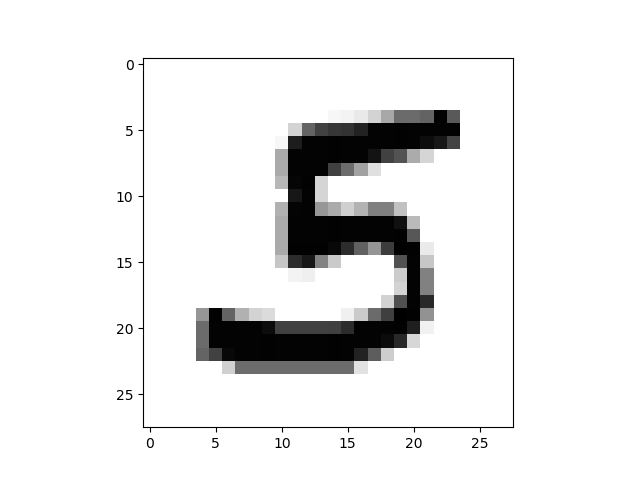
\includegraphics[width=\textwidth]{img786render.png}
    \end{minipage}
    \begin{minipage}[t]{0.3\textwidth}
        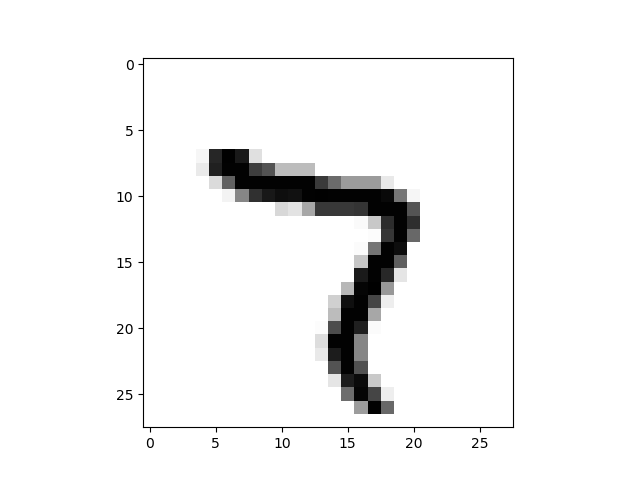
\includegraphics[width=\textwidth]{img98render.png}
    \end{minipage}
    \begin{minipage}[t]{0.3\textwidth}
        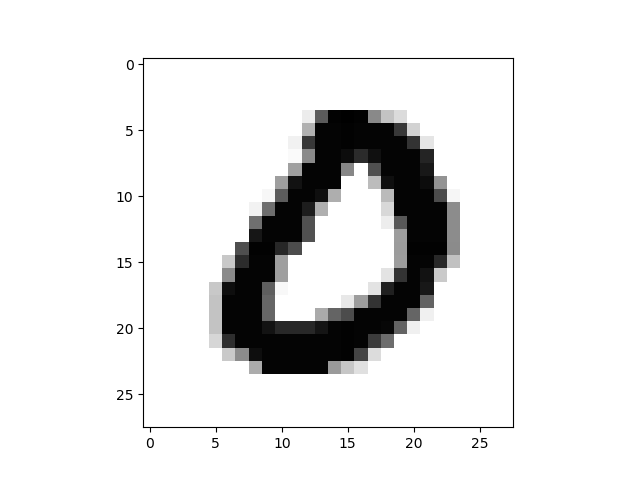
\includegraphics[width=\textwidth]{img6render.png}
    \end{minipage}
  \caption{Image Renderings from the MNIST Dataset}
\end{figure}
\section{Random Forest}
A Random Forest (RF) is a common starting algorithm for those new to machine learning. This is in part due to it's easy of use, but also due to it's flexibility. While in this assignment it is used for classification, it can be also be used in regression problems. Each tree is formed from a bootstrap sample (random sampling with replacement) then grown very similarly to a decision tree. Rather than searching for the very best split feature, it chooses the best of a random subset. Unlike the standard RF algorithm, \verb+sklearn+'s \verb+RandomForestClassifier+ combines the probabilistic prediction of each tree, rather than picking a classification based on a majority vote. 

These models are generally very fast to train, but depending on the complexity, can suffer from slow run-time performance. Generally speaking, overfitting can be negated by simple adding more trees to your model. This approach eventually results in diminishing returns, and for high-dimensional problems such as digit recognition, is especially impractical.

\subsection{Implementation}
The 784 length vector of input data is normalized to range from 0 to 1 using \verb+sklearn+'s \verb+preprocessing.minmax_scale+. In order to improve our model's predictive power, we contrasted the results from our hyperparameters \verb+n_estimators+ (number of trees) and  \verb+min_samples_split+ (minimum number of leafs required to split a node). Specifically we allowed 10, 50, 100, and 300 trees to be developed and 2, 4, 8, and 16 as the minimum number of leafs. The later can be thought of as a measure of complexity, with lower minimum resulting in higher complexity. Once the code was prepared, training took approximately 45 minutes. 
\begin{figure}[h]
    \centering
    \begin{minipage}[t]{0.45\textwidth}
        \centering
        \textbf{(A)}
        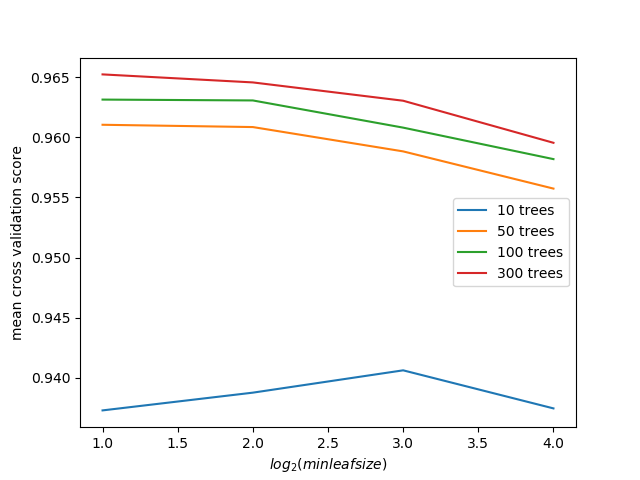
\includegraphics[width=\textwidth]{CVscoreVsLeafSize.png}
    \end{minipage}
    \begin{minipage}[t]{0.45\textwidth}
        \centering
        \textbf{(B)}
        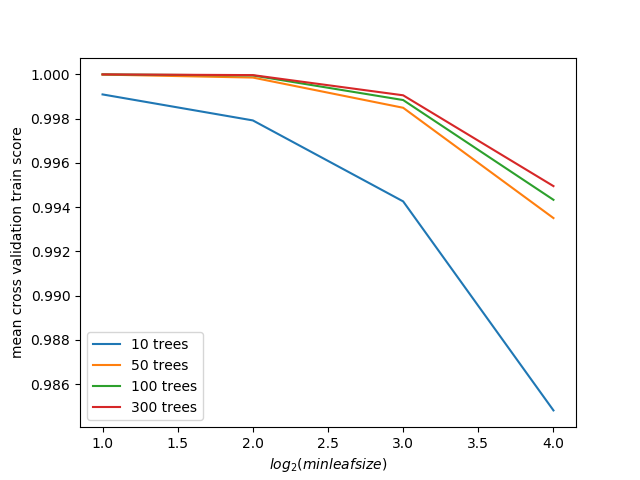
\includegraphics[width=\textwidth]{CVtestVsLeafSize.png}
    \end{minipage}
\caption{(A,B) Cross Validation of Hyperparameters for (A) training data and (B) testing data by contrasting mean cross validation score and $\log_2(minleafsize)$ giving the minimum leaf threshold as a measure of complexity. The scores for varying numbers of trees are shown.}
\end{figure}
\section{Random Forest}

\subsection{Cross-Validation and Results}
Training and cross-validation was done using \verb+model_selection.GridSearchCV+. In order to visualize the results, Figure 2 contrasts the prediction rates of the training and test datasets. The $\log_2(minleafsize)$ which inversely measures the complexity suggests the more complex models preform outstandingly against the training data but have little impact on the testing data. Adding trees has a similar positive affect on both datasets, however, also decreases exponentially as more trees are added. These results suggest that our model suffers from extreme levels of overfitting. As expected, adding trees does improve our models predictive power but isn't the most practical for our dataset. Our Kaggle submission gave a prediction rate of 96.6\%

\section{Multi-Layer Perceptron Classifier}
This will be much more interesting to talk about

\subsection{Contrasting Gradient Descent Algorithms}
Because it will probably be good to talk about why Adam's so good, basically because it used the components of a lot of other good methods.

\subsection{Implementation}

\subsection{Cross-Validation and Results}

\section{Conclusions}

\clearpage

\section*{References}

References follow the acknowledgments. Use unnumbered first-level heading for
the references. Any choice of citation style is acceptable as long as you are
consistent. It is permissible to reduce the font size to \verb+small+ (9 point)
when listing the references. {\bf Remember that you can use more than eight
  pages as long as the additional pages contain \emph{only} cited references.}
\medskip

\small

[1] Alexander, J.A.\ \& Mozer, M.C.\ (1995) Template-based algorithms for
connectionist rule extraction. In G.\ Tesauro, D.S.\ Touretzky and T.K.\ Leen
(eds.), {\it Advances in Neural Information Processing Systems 7},
pp.\ 609--616. Cambridge, MA: MIT Press.

[2] Bower, J.M.\ \& Beeman, D.\ (1995) {\it The Book of GENESIS: Exploring
  Realistic Neural Models with the GEneral NEural SImulation System.}  New York:
TELOS/Springer--Verlag.

[3] Hasselmo, M.E., Schnell, E.\ \& Barkai, E.\ (1995) Dynamics of learning and
recall at excitatory recurrent synapses and cholinergic modulation in rat
hippocampal region CA3. {\it Journal of Neuroscience} {\bf 15}(7):5249-5262.

\end{document}
